% Gemini theme
% https://github.com/anishathalye/gemini

\documentclass[final]{beamer}

% ====================
% Packages
% ====================

\usepackage[T1]{fontenc}
\usepackage{lmodern}
\usepackage[orientation=portrait,size=a0,scale=1.5]{beamerposter}
\usetheme{gemini}
\usecolortheme{mit}

\usepackage{bm}
\usepackage{graphicx}
\usepackage{booktabs}
\usepackage{tikz}
\usepackage{pgfplots}
\pgfplotsset{compat=1.14}
\usepackage{anyfontsize}

% ====================
% Lengths
% ====================

% If you have N columns, choose \sepwidth and \colwidth such that
% (N+1)*\sepwidth + N*\colwidth = \paperwidth
\newlength{\sepwidth}
\newlength{\colwidth}
\setlength{\sepwidth}{0.04\paperwidth}
\setlength{\colwidth}{0.44\paperwidth}

\newcommand{\separatorcolumn}{\begin{column}{\sepwidth}\end{column}}

% ====================
% Title
% ====================

\title{\huge{Solving generic parametric linear matrix inequalities}}

\author{Simone Naldi\inst{1} \and Mohab Safey El Din\inst{2} \and Adrien Taylor\inst{3} \and Weijia Wang\inst{2}}

\institute[shortinst]{\inst{1} Université de Limoges, CNRS, XLIM, Limoges, France \\ \inst{2} Sorbonne Université, CNRS, LIP6, Paris, France \\ \inst{3} Inria, École normale supérieure, PSL Research University, Paris, France }

% ====================
% Footer (optional)
% ====================

\footercontent{
  
\includegraphics[height=3cm]{images/unilim.png} \hfill
  
\includegraphics[height=3cm]{images/cnrs.png} \hfill
  
\includegraphics[height=3cm]{images/xlim.png} \hfill
  
\includegraphics[height=3cm]{images/su.png} \hfill
  
\includegraphics[height=3.2cm]{images/lip6.png} \hfill
  
\includegraphics[height=3cm]{images/inria.png} \hfill
  
\includegraphics[height=3cm]{images/ens-psl.png}
}
% (can be left out to remove footer)

% ====================
% Logo (optional)
% ====================

% use this to include logos on the left and/or right side of the header:
% \logoright{\includegraphics[height=7cm]{logo1.pdf}}
% \logoleft{\includegraphics[height=7cm]{logo2.pdf}}

% ====================
% Body
% ====================

\usepackage{subcaption}
\usepackage[dvipsnames]{xcolor}

\newcommand{\citeauthorandyear}[2]{\textcolor{gray}{[#1 #2]}}

\begin{document}

\begin{frame}[t]
    \begin{columns}[t]
        \separatorcolumn

        \begin{column}{\colwidth}

            \begin{block}{Parametric linear matrices}
                Let $\bm{y}=(y_1,\ldots,y_t)$, $\bm{x}=(x_1,\ldots,x_n)$.

                $f\in\mathbb{Q}[\bm{y}][\bm{x}]_{\leq 1}$ = linear polynomial in $\bm{x}$ parametric in $\bm{y}$

                $A\in\mathbb{S}_{m}(\mathbb{Q}[\bm{y}][\bm{x}]_{\leq 1})$ = parametric linear matrix

                \begin{figure}
                    \begin{subfigure}{.5\textwidth}
                        \centering
                        \begin{equation*}
                            A(y,x) =
                            \begin{bmatrix}
                                y_1 y_2   & x_1     & y_2^3 x_2 \\
                                x_1       & y_2+y_3 & y_1 x_3   \\
                                y_2^3 x_2 & y_1 x_3 & y_1^2+y_3
                            \end{bmatrix}
                        \end{equation*}
                        \vspace{2cm}
                    \end{subfigure}%
                    \begin{subfigure}{.5\textwidth}
                        \centering
                        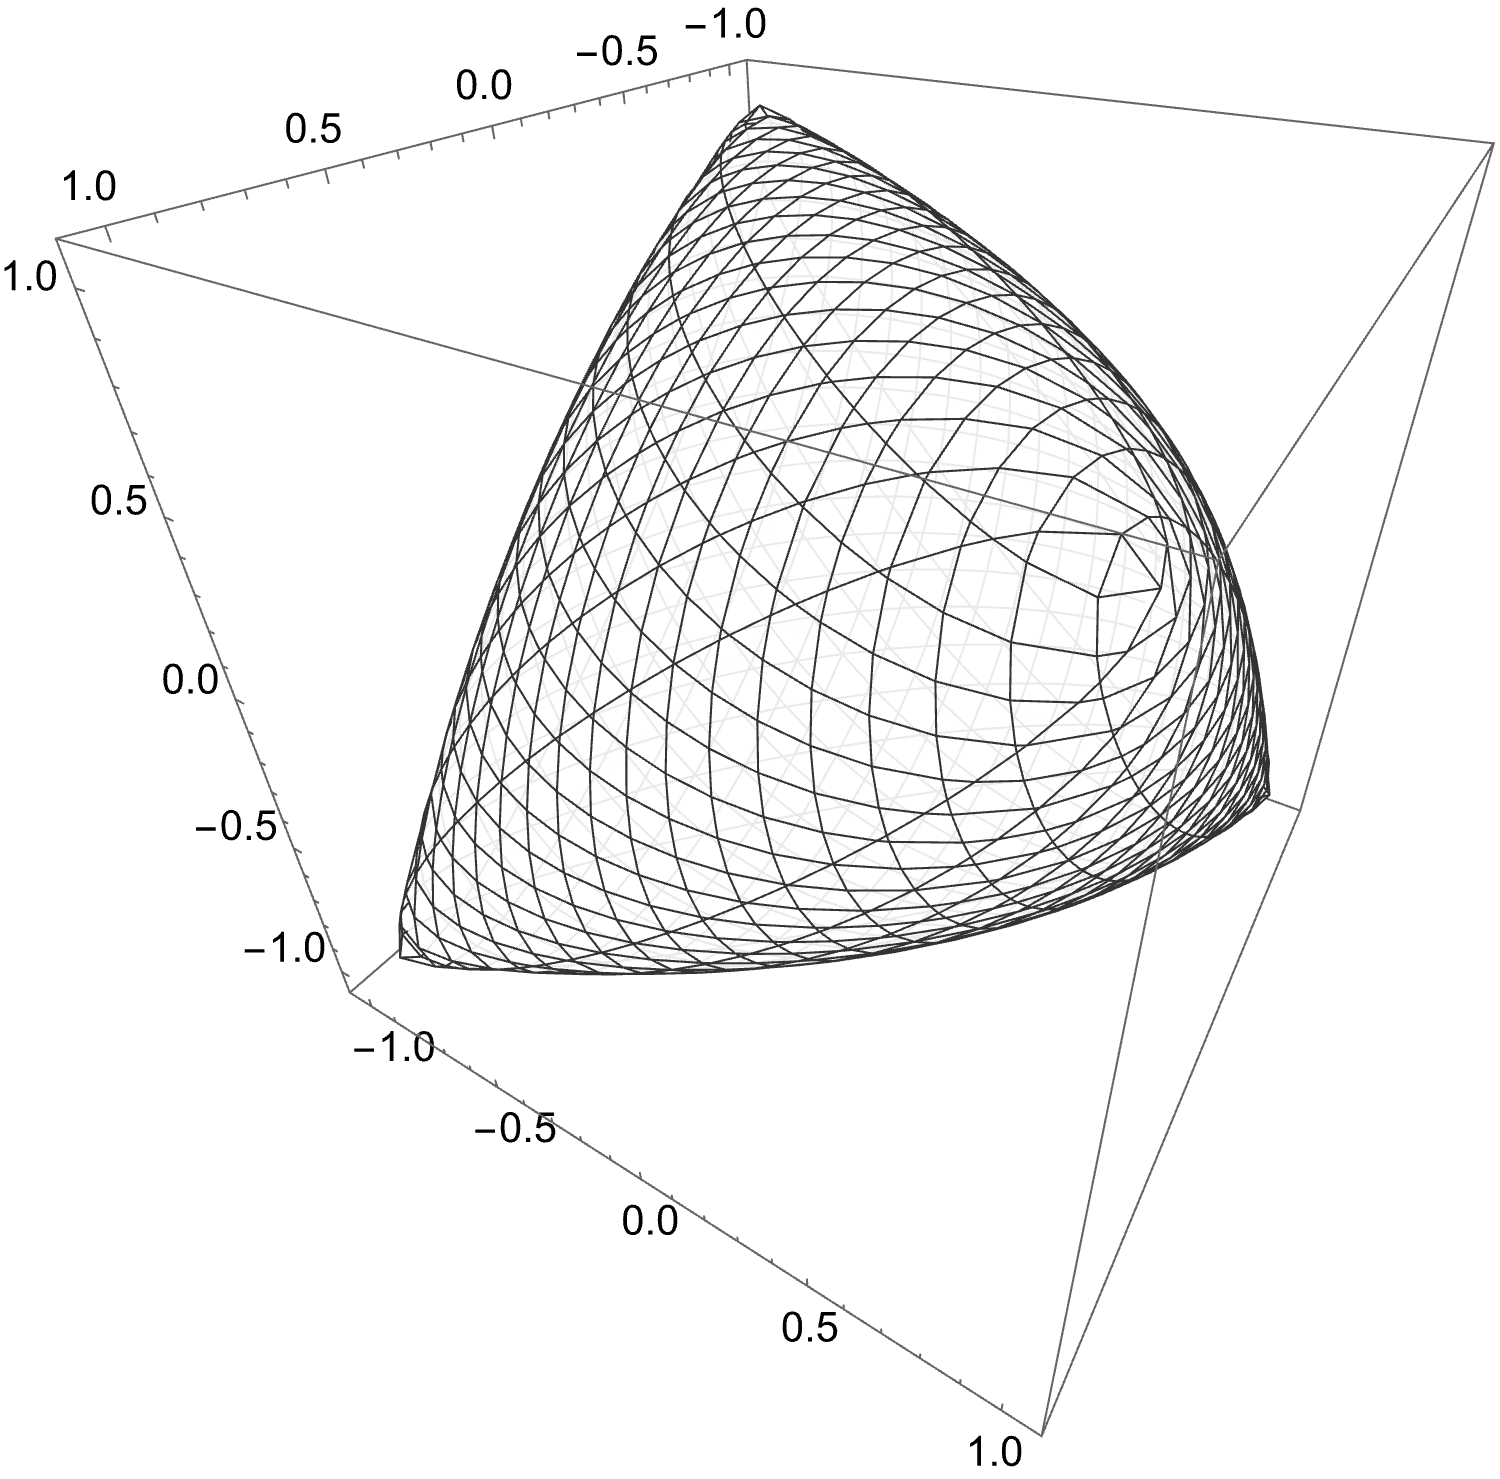
\includegraphics[height=8cm]{images/spectrahedron.png}
                    \end{subfigure}
                    \vspace{-2cm}
                    \caption{Spectrahedron $\lbrace x\in\mathbb{R}^{3}:A(y,x)\succeq 0\rbrace$, with $y=(1,1,0)$}
                \end{figure}
            \end{block}

            \begin{alertblock}{Problem}
                Let $A\in\mathbb{S}_{m}(\mathbb{Q}[\bm{y}][\bm{x}]_{\leq 1})$,
                and $\mathcal{P}$ be the set of parameters $y\in\mathbb{R}^t$
                such that the parametric \textbf{linear matrix inequality} (LMI)
                \begin{equation*}
                    A(y,\cdot)\succeq 0
                \end{equation*}
                is feasible, i.e. for some $x\in\mathbb{R}^n$,
                $A(y,x)$ is positive semidefinite /
                only has nonnegative eigenvalues.

                \textbf{Goal}: extract a formula $\Phi$ describing
                (a dense subset of) $\mathcal{P}$

                \begin{figure}[H]
                    \centering
                    \begin{tikzpicture}[every node/.style={align=center}]
                        \node (A) at (0, 0) {$A \succeq 0$};
                        \node (B) at (22, 0) {$\Phi$};
                        \node (C) at (0, -4.5) {$A(y,\cdot) \succeq 0$};
                        \node (D) at (22, -4.5) {$\Phi(y)$};
                        \draw[->] (A) -- (B) node[midway, above] {\small{\citeauthorandyear{Naldi-Safey El Din-Taylor-W}{2025}}};
                        \draw[->, dashed] (A) -- (C) node[midway, left] {\textcolor{Brown}{specialize}};
                        \draw[->, dashed] (C) -- (D) node[midway, below] {\small{\citeauthorandyear{Henrion-Naldi-Safey El Din}{2016}}};
                        \draw[->, dashed] (B) -- (D) node[midway, right] {\textcolor{Brown}{specialize}};
                    \end{tikzpicture}
                \end{figure}
            \end{alertblock}

            \begin{block}{Applications}
                \begin{itemize}
                    \item Parametric sum-of-squares problem

                          \citeauthorandyear{Motzkin}{1967}
                          \citeauthorandyear{Robinson}{1973}
                    \item Convergence analyses of first-order optimization methods

                          \citeauthorandyear{Drori-Teboulle}{2014}
                          \citeauthorandyear{Taylor-Hendrickx-Glineur}{2018}
                          \citeauthorandyear{Kim-Fessler}{2021}
                          \citeauthorandyear{Lieder}{2021}
                          \citeauthorandyear{Drori-Taylor}{2023}
                \end{itemize}
            \end{block}

            \begin{exampleblock}{Quantifier Elimination?}
                Let $g_0,\ldots,g_m$ be
                the coefficients
                of $\det(A+\lambda I_{m})$ in $\lambda$. Then,
                \begin{equation*}
                    A(y,x)\succeq 0 \iff g_0(y,x)\geq 0 \land \ldots \land g_m(y,x)\geq 0.
                \end{equation*}
                Compute $\Phi$ = eliminate $\exists x$ in the formula (QE)
            \end{exampleblock}

            \begin{block}{Contributions}
                \begin{figure}[H]
                    \centering
                    \begin{tikzpicture}[every node/.style={align=center}]
                        \node (A) at (0, 0) {\textbf{Input} \\ Parametric LMI};
                        \node (B) at (24, 0) {\textbf{Output} \\ Feasibility formula};
                        \node (C) at (12, -12) {0-dim systems in $\mathbb{Q}(\bm{y})[\bm{x},\ldots]$};

                        \draw[->, dashed] (A) -- (B) node[midway, above] {Quantifier elimination};
                        \draw[->] (A) -- (C) node[midway, left=12mm] {\textcolor{Maroon}{Parametric} \\ \textcolor{Maroon}{SolveLMI} \\ \small{\textcolor{gray}{[Naldi-Safey El Din-}} \\ \small{\textcolor{gray}{Taylor-W 2025]}}};
                        \draw[->] (C) -- (B) node[midway, right=9mm] {\textcolor{Maroon}{Real root} \\ \textcolor{Maroon}{classification} \\ \small{\textcolor{gray}{[Gaillard-Safey El Din}} \\ \small{\textcolor{gray}{2024]}}};
                    \end{tikzpicture}
                    \caption{Algorithmic pipeline}
                \end{figure}
            \end{block}
        \end{column}

        \separatorcolumn

        \begin{column}{\colwidth}
            \begin{exampleblock}{State of the Art}
                \begin{itemize}
                    \item CAD: doubly exponential in $n$
                          \citeauthorandyear{Collins}{1975}
                    \item Border polynomials

                          \citeauthorandyear{Yang-Xia}{2005}
                          \citeauthorandyear{Liang-Jeffrey-Maza}{2008}
                          \citeauthorandyear{Moroz}{2006}
                          \citeauthorandyear{Lazard-Rouillier}{2007}
                          \citeauthorandyear{Le-Safey El Din}{2022}
                \end{itemize}
            \end{exampleblock}

            \begin{block}{Parametric SolveLMI}
                \begin{figure}[H]
                    \begin{tikzpicture}[every node/.style={align=center}]
                        \node (A) at (0, 0) {Parametric LMI};
                        \node (B) at (20, 0) {0-dim systems in $\mathbb{Q}(\bm{y})[\bm{x},\ldots]$};
                        \node (C) at (0, -7.5) {Parametric \\ determinantal varieties};
                        \node (D) at (20, -7.5) {Parametric sample points \\ in each connected component};
                        \node (E) at (0, -15) {Determinantal \\ varieties};
                        \node (F) at (20, -15) {Sample points \\ in each connected component};

                        \draw[->] (A) -- (B) node[midway, above] {\textcolor{Maroon}{Parametric} \\ \textcolor{Maroon}{SolveLMI}};
                        \draw[->] (A) -- (C) node[midway, right] {\textcolor{Maroon}{rank stratification}};
                        \draw[->] (C) -- (D) node[midway, above] {};
                        \draw[<->] (D) -- (B) node[midway, right] {\textcolor{Maroon}{parametrization}};
                        \draw[->, dashed] (C) -- (E) node[midway, right] {\textcolor{Brown}{specialize}};
                        \draw[->, dashed] (D) -- (F) node[midway, right] {\textcolor{Brown}{specialize}};
                        \draw[->, dashed] (E) -- (F) node[midway, below] {\textcolor{Brown}{SolveLMI} \\ \small{\citeauthorandyear{Henrion-Naldi-Safey El Din}{2016}}};
                    \end{tikzpicture}
                    \caption{Reduction to zero-dimensional systems}
                \end{figure}
            \end{block}

            \begin{alertblock}{Arithmetic Complexity}
                For generic $A\in\mathbb{S}_{m}(\mathbb{Q}[\bm{y}]_{\leq d}[\bm{x}]_{\leq 1})$,
                \# of operations in $\mathbb{Q}$:
                {
                \large
                \begin{equation*}
                    2^{O(mt)}n^{O(1)}(md)^{O(t)}(\upperbound{\delta}\upperbound{\Delta})^{O(t)}
                \end{equation*}
                }
                where
                \begin{align*}
                    \upperbound{\delta}  \in n^{O(m^2)}\quad  \text{ and } \quad
                    \upperbound{\Delta}  \in e^{O(m^2\log m)}n^{O(1)}d^{O(m^2+t)}t^{O(1)}.
                \end{align*}

                \textbf{Complexity}: polynomial in $n$ when $m$ is fixed
            \end{alertblock}

            \begin{block}{Benchmark}
                \begin{itemize}
                    \item First implementation in Maple, with calls to msolve
                          \citeauthorandyear{Berthomieu-Eder-Safey El Din}{2021}
                \end{itemize}

                \begin{table}
                    \centering
                    \begin{tabular}{l r r r c}
                        \toprule
                                       & \textbf{RRC} & \textbf{RRC sig} & \textbf{QE/Maple} & \textbf{QE/Wolfram} \\
                        \midrule
                        \textsf{MKN11} & 5.0 s        & 1.5 s            & 5.7 s             & 0.06 s              \\
                        \textsf{RBN11} & 5.0 s        & 1.6 s            & 7.1 s             & 0.04 s              \\
                        \textsf{GRD12} & 1.0 s        & 3.7 s            & $\infty$          & 0.5 s               \\
                        \textsf{GRD13} & 19 s         & 17 s             & $\infty$          & $\infty$            \\
                        \textsf{GRD14} & $\infty$     & $\infty$         & $\infty$          & $\infty$            \\
                        \textsf{GRD21} & 0.5 s        & 1.7 s            & 1.3 s             & 0.1 s               \\
                        \textsf{GRD22} & 5.8 s        & 2 min            & $\infty$          & 42 min              \\
                        \textsf{GRD23} & $\infty$     & $\infty$         & $\infty$          & $\infty$            \\
                        \textsf{PPM21} & 0.3 s        & 0.3 s            & 0.3 s             & 0.005 s             \\
                        \textsf{PPM31} & 0.3 s        & 0.4 s            & 0.4 s             & 0.007 s             \\
                        \textsf{DRS32} & 2.2 s        & 8 h              & $\infty$          & $\infty$            \\
                        \textsf{DRS33} & 18 min       & $\infty$         & $\infty$          & $\infty$            \\
                        \textsf{DRS42} & 52 s         & $\infty$         & $\infty$          & $\infty$            \\
                        \textsf{DRS43} & $\infty$     & $\infty$         & $\infty$          & $\infty$
                        \bottomrule
                    \end{tabular}
                    \caption{Benchmark results}
                \end{table}

            \end{block}

        \end{column}

        \separatorcolumn
    \end{columns}
\end{frame}

\end{document}
